\chapter{Grundlegende Begriffe}
\label{ch:basics}
In folgendem Kapitel werden die Grundlagen erläutert, welche für spätere Kapitel benötigt werden. 
Es wird kurz auf die Historie von Turing Tests eingegangen, 
bevor die verschiedenen CAPTCHA-Methoden und Alternativen grundlegend erläutert werden. 
Zuletzt wird ein grundlegendes Verständnis für UX geschaffen.

\section{Turing Tests}
\label{ch:basics:turing}
Alan M. Turing $($1912-1954$)$ ist einer der Mitbegründer der heutigen Informatik 
und legte mit seiner Forschung einen der Grundsteine für die Entwicklung von künstlicher Intelligenz. 
In seinem Paper ''On computable numbers, with an application to the Entscheidungsproblem'' \cite{turing} 
beschreibt er den Umgang mit ''computable numbers'' und wie diese durch eine - später als Turing Machine bezeichnete - Maschine berechnet werden könnte.
Diese Turing Machine ''[\dots] ist damit ein Model physischer digitaler Computer, die zu jener Zeit jedoch noch nicht existieren. [\dots]'' \cite[p.4]{pallay2020turing}
Hierbei kam er zur Erkenntnis, dass sich nicht alle mathematischen Probleme durch eine fixe Vorgehensweise, also einen Algorithmus, lösen lassen. 
Erst später wurde festgestellt, dass Turing Maschinen und Computer jeweils vom anderen simuliert werden können. \cite[p.647]{geniusofturing} \cite[p.4]{pallay2020turing} %TODO: Formulierung

Turing beschäftigte sich bis zu seinem frühen Tod weiterhin mit maschineller Intelligenz 
und ''[\dots] beschreibt [\dots] das, was man heute als [\dots] künstliche Intelligenz bezeichnet.'' \cite[p.10]{pallay2020turing}
Durch seine Überzeugung, dass eines Tages maschinelle Intelligenzen entwickelt werden (können), 
entwickelte Turing in seinem Paper ''Computing Machinery and Intelligence'' \cite[p.23ff]{turing2009computing} 
eine Methode des Testens der Intelligenz einer Maschine. 
Um die Notwendigkeit von genauen Definitionen zu vermeiden, nutzt er deshalb ein Abwandlung eines Verfahren - des ``imitation games''. 
''Hierbei kommuniziert ein Juror maschinen-schriftlich mit einem Menschen und einer Maschine.'' \cite[p.12]{pallay2020turing}
Sollte der Juror nicht feststellen können, welcher Gesprächspartner der Mensch ist, gilt der Test als bestanden. \cite[p.11ff]{pallay2020turing}

Dieses Verfahren wird heute oftmals als Turing Test bezeichnet. 

\section{CAPTCHA}
\label{ch:basics:captcha}
Bei der Abkürzung CAPTCHA handelt es sich um ''completely automated public turing tests to tell computers and humans apart''. 
Sie werden genutzt, um Webseiten vor Angriffen durch Bots zu schützen. 
Dies wird durch die im vorherigen Kapitel bereits erläuterten Turing Tests erreicht. 
Hier ist das Ziel, durch für Computer schwer, für Menschen jedoch leicht zu verarbeitende Medien, das Tracken von Mausbewegungen
oder das Prüfen der Browseraktivität zu prüfen, ob es sich wirklich um eine*n menschliche*n Nutzer*in handelt.

Fast identisch zu CAPTCHA sind sogenannte HIP – ''Human Interactive Proofs''. 
Dieser Begriff hat sich entwickelt, da manche Tests nicht ''public'' sind. \cite[p.1]{chellapilla} \cite{tutorial} 

\subsection{Arten von CAPTCHA}
\label{ch:basics:captcha:arten}
%Nachfolgend werden verschiedene Arten von CAPTCHAs grundlegend erläutert.
Textbasierte CAPTCHA waren bereits 2008 die am häufigsten verwendete Art von CAPTCHA.
Sie zeichnen sich durch eine Verzerrung eines Wortes oder mehreren Wörtern aus, sodass diese für Bilderkennungstools nicht erkennbar sind.
Eine weitere Variante textbasierter CAPTCHA ist die einer einfachen Rechenaufgabe. 
Auch hier soll erreicht werden, dass ein Bot die angegebenen Zahlen nicht korrekt erkennen kann und die Gleichung somit nicht lösen kann. \cite{usabilityofcaptchas} \cite[p.75]{surveyofresearch} \cite{shinde2018DIFFERENTTO} %TODO SEITEN!!!!!!!!!

Bei der Darstellung dieser Zeichen und Symbole können verschiedene Ansätze verfolgt werden.
\citeauthor{surveyofresearch} beschreiben hierbei ``anti-segmentation techniques'' und ``anti-recognition techniques''. \cite[p.76]{surveyofresearch}

Anti-Segmentation Techniques zielen darauf ab, das Separieren der einzelnen Buchstaben durch Algorithmen zu erschweren. 
Um dies zu erreichen, gibt es verschiedene Herangehensweise.
Eine von ihnen besteht daraus, dass nur die Konturen der verschiedenen Zeichen angezeigt werden, sodass diese nur von Menschen erkannt werden können,
Bots hingegen wenig Chancen haben, diese korrekt zu unterscheiden. Diese Art von CAPTCHA nennen \citeauthor[p.76]{surveyofresearch} ``Hollow CAPTCHAs''. %Formulierung
Eine weitere Methode ist, Zeichen nah beieinander oder sogar überlappend darzustellen, 
was von \citeauthor{surveyofresearch} als ``crowing characters together $($CCT$)$ and overlapping'' bezeichnet wird.
Auch unruhige Hintergründe können Segmentierung behindern.
Ebenfalls beschrieben wird die Kombination von mehreren der beschriebenen CAPTCHAs zu einer ``two-layer'' Struktur,
wobei die Tatsache, dass es sich um mehrere Zeilen Text handelt, nicht erkannt werden kann. \cite[p.76]{surveyofresearch}

Anti-Recognition Techniques sind zum Beispiel verschiedene Schriftarten, die Rotation von Zeichen und ``Waving'', 
welche es erschweren, Zeichen als solche zu erkennen. 
Außerdem können in einigen Fällen auch sehr große Zeichensätze, beispielsweise Mandarin oder Japanisch, genutzt werden, 
wodurch das Finden von eindeutigen Lösungen erschwert werden kann.
Diese Techniken werden oftmals miteinander kombiniert.
\cite[p.77]{surveyofresearch}

\begin{figure}
    \centering
    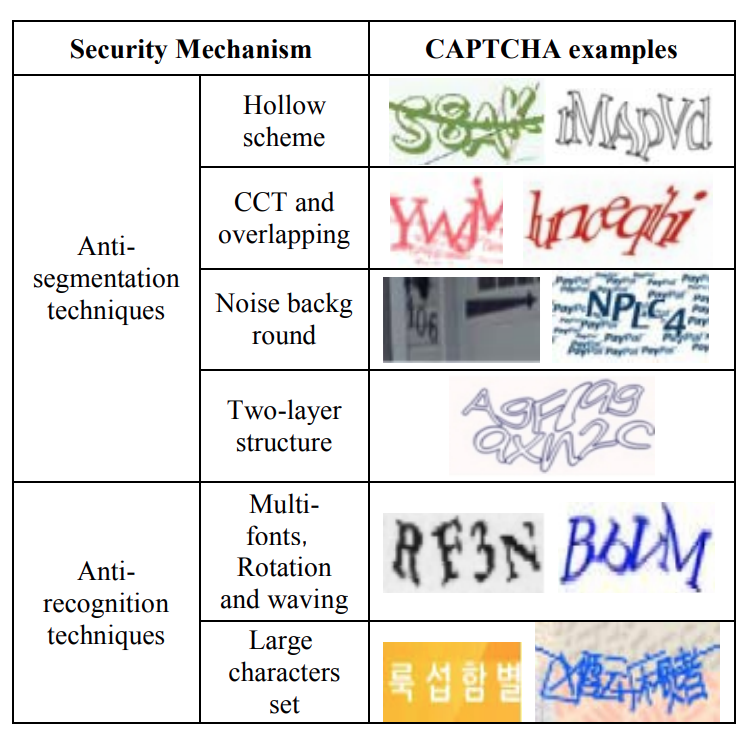
\includegraphics{gfx/mygraphics/unbedingtaustauschen1.png}
    \caption{textbasierte Beispiele die ich unbedingt noch austauschen muss, weil sie aus \cite{surveyofresearch} sind}
\end{figure}

Es gibt verschiedene Arten von bildbasierten CAPTCHAs. 
Die wohl bekannteste ist ein in Quadrate aufgeteiltes Bild, wobei man jene Quadrate auswählen soll, welche einen bestimmten Gegenstand enthalten.
Eine Variation dieses CAPTCHAs besteht aus einer Zahl verschiedener Bilder, von denen eine Teilmenge ebenfalls ein gesuchtes Objekt beinhalten -
sogenannte ``Semantically Matching Images''. \cite[p.xx]{surveyofresearch}
In Abbildung \ref{fig:fortnite} sollen Hunde mit geschlossenen Augen ausgewählt werden,
was die Notwendigkeit der Zunahme der Komplexität dieser CAPTCHAs gut widerspiegelt. 
Außerdem kann auch auf das Erkennen von Gesichtern durch Menschen gesetzt werden.
Nähere Informationen zu genauen Techniken können in \cite[p.xx]{surveyofresearch} nachgelesen werden.
Die beschriebenen ``selection-based CAPTCHA'' bezeichnen \citeauthor{surveyofresearch} als einfachste Form bildbasierter CAPTCHA.

In Abbildung \ref{fig:genshin} sind zwei weitere Arten bildbasierter CAPTCHA dargestellt.
Links ist ein ``drag-based CAPTCHA'' dargestellt.
Hierbei werden Mausbewegungen, die Geschwindigkeit dieser Bewegungen
und die allgemeine Reaktionszeit überprüft.
Dies geschieht, wie in Abbildung \ref{fig:genshin} (a) zu sehen,
beispielsweise über das Verschieben eines Puzzleteils an die richtige Stelle.
Auch hier kann in \cite[p.xx]{surveyofresearch} genauer nachgelesen werden.

%Discord CAPTCHA: PFERDE AUS WOLKEN!!!!!
%Eine Form von bildbasierten sind Gamification captcha
%B. Click-based CAPTCHA
%In 2008, Richard Chow et al.[23] first proposed the clickbased CAPTCHA. It requires users to click characters in a
%complex background according to a short hint, as shown in
%Fig. 3. This CAPTCHA simplifies the user's operation,
%shortens the passing time and minimizes users’ frustration.
%Fig. 3. Examples of click-based CAPTCHAs
%In general, click-based CAPTCHAs have two defense
%mechanisms: anti-detection and anti-recognition. It is no
%longer a difficult task to recognize characters correctly with
%the development of machine learning. Therefore, almost all
%security mechanisms focus on preventing attackers from
%77
%Authorized licensed use limited to: Fachhochschule FH Darmstadt. Downloaded on July 29,2022 at 08:34:41 UTC from IEEE Xplore. Restrictions apply.
%correctly detecting characters. As shown in Fig. 3(c), the
%CAPTCHA uses the style transfer technique [24] to embed
%characters into the background to achieve the effect of hiding
%the characters.
%Recently, a novel click-based CAPTCHA named VTT was
%proposed by Tencent (see Fig. 4). For a computer, it is
%difficult to understand the semantic information and analyze
%the image content as well as humans. In this regard, it seems a
%good design. However, state-of-the-art research on visual
%reasoning, such as [58] and [8], may break this scheme in the
%near future.
%Fig. 4. Examples of VTT CAPTCHAs


\begin{figure}
    \centering
    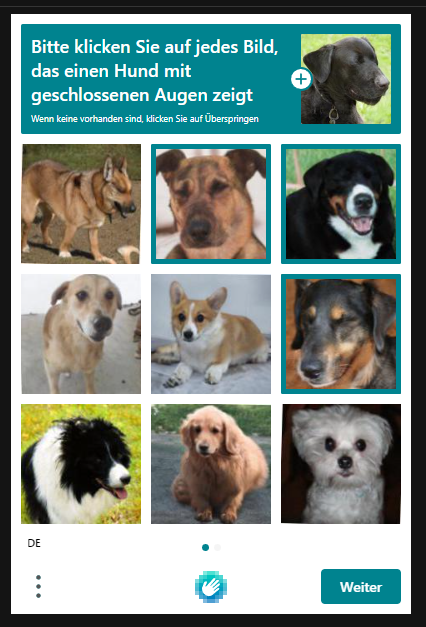
\includegraphics{gfx/mygraphics/fuerfortnite.png}
    \caption{Bildbasierter CAPTCHA bei Login auf der Epic Games Website}   
    \label{fig:fortnite}
\end{figure}

% Gamification
\cite{gamified}

\begin{figure}
    \centering
    \subfloat[\centering]{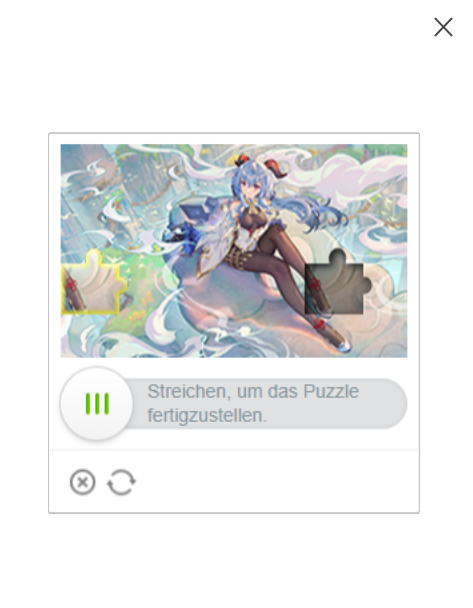
\includegraphics[width=5cm]{gfx/mygraphics/genshincaptcha.png}}
    \qquad
    \subfloat[\centering]{
\includegraphics[width=5cm]{gfx/mygraphics/hoyoversecaptcha.png}}
    \caption{Bildbasierte CAPTCHA bei Login in Genshin Impact $($a$)$ und dem Forum Hoyolab $($b$)$}   
    \label{fig:genshin}
\end{figure}

%Videobasiert
Eine weitere Form visueller CAPTCHAs sind videobasierte CAPTCHA. 
Nutzer*innen müssen beispielsweise verschiedene Bewegungen erkennen, die im Video ausgeführt werden,
oder auch angezeigte Werbung.
Dabei werden verschiedene Antwortmöglichkeiten vorgegeben, welche durch Raten auch durch Bots erfolgreich absolviert werden können.
Um dies zu umgehen gibt es Alternativen, die über das Beschreiben des gesehenen Videos funktionieren. \cite[p.xx]{surveyofresearch} 

%Audiobasiert
Als Alternative von visuellen CAPTCHAs können audiobasierte CAPTCHA genutzt werden.
Diese bieten sich vor allem für sehbehinderte Nutzer*innen an, welche bild- oder textbasierte CAPTCHA nur schwer oder gar nicht sehen und erkennen können.
Oft wird hier Text-To-Speech verwendet, wobei die gehörten Wörter durch die Nutzer*innen wiederholt werden sollen.
Eine weitere Möglichkeit ist das Abspielen bestimmter Töne, wie die einer Glocke oder eines Klaviers. 
Die kann auch in Kombination mit verschiedenen Hintergrundgeräuschen angewandt werden, was das Erkennen eines bestimmten Tons für Roboter zusätzlich erschwert.
Außerdem gibt es Methoden, bei denen eine bestimmte Frage beantwortet werden muss, für die ``common sense'' $($dt. ``Gesunder Menschenverstand''$)$ notwendig ist.
Neben Techniken, die hauptsächlich auf das Hören ausgelegt sind, kann der Fokus auch auf das Einsprechen von Phrasen durch die Nutzer*innen gelegt werden.
Es soll so erkannt werden, ob es sich um eine menschliche Stimme handelt.
\cite[p.78]{surveyofresearch}

Eine aktuell viel genutzte Form der Spam-Prävention ist reCAPTCHA v3 von Google. 
Hier werden keine Turing Tests durchgeführt. 
Vielmehr wird anhand verschiedener Faktoren bewertet, ob es sich um einen Bot oder einen Menschen handelt.
Was genau diese Faktoren sind, gibt Google aus Sicherheitsgründen nicht Preis. 
Denkbar ist jedoch die Betrachtung von Cookies oder der Häufigkeit von Anfragen durch die gegebene IP-Adresse.
In der Dokumentation wird angegeben, dass ein Score von 0.0 bis 1.0 vergeben werden kann. 
Hier gilt: Je niedriger der Score, desto wahrscheinlicher handelt es sich um einen Bot statt eines ``echten'' Nutzers. (Vgl. \cite{recaptchadoc})
Laut Google selbst soll reCAPTCHA v3 eine sehr gute Nutzererfahrung bieten, da es kaum bis gar keine Zuarbeit durch den Nutzer verlangt. \cite{googleblog:recaptcha}
ReCAPTCHA kann durch das Fehlen eines klassischen Turing Tests auch als eine CAPTCHA-Alternative interpretiert werden.

\begin{figure}
    \centering
    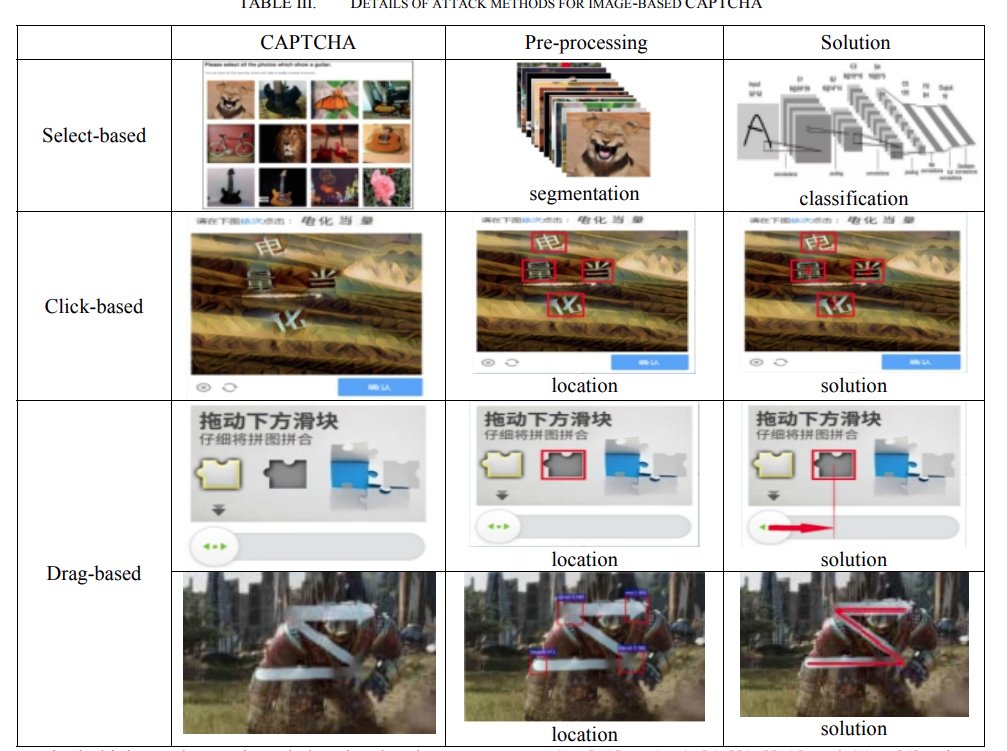
\includegraphics{gfx/mygraphics/unbedingtaustauschen2.png}
    \caption{bildbasierte Beispiele die ich unbedingt noch austauschen muss, weil sie aus \cite{surveyofresearch} sind}
    \label{fig:pr0grammcaptcha}
\end{figure}

\subsection{Alternativen zu klassischen CAPTCHA}
%anti spam plugins
%multi faktor authentifikation
%biometrie
Eine weitere Alternative zu klassischen CAPTCHA sind sogenannte Honeypots. 
Geprägt wurde der Begriff erstmals im Kalten Krieg als Spionagetechnik eingesetzt wurde. \cite[p.2]{joshi:2011} 

Auch heute werden Honeypots eingesetzt, und zwar in der IT-Sicherheit. 
Oft werden sie mit ``Fallen'' assoziiert, welche Hacker anlocken sollen. 
Dadurch können Angriffsarten analysiert werden und ''echte'' Systeme werden nicht angegriffen.

Doch auch im Kontext der Unterscheidung von Menschen und Maschine gibt es Honeypots. 
So kann man HTML-Inputfelder durch CSS verstecken, sodass diese nur durch Bots, welche den Quellcode der Seite scannen, ausgefüllt werden 
und nicht durch Menschen, da diese das Textfeld nicht sehen. 
Bei der Prüfung der Inputs kann nun überprüft werden, ob ein Bot in die Falle getappt ist. 
Nachzulesen sind solche Verfahren in verschiedenen Blogposts, wie \cite{perry:2019}.


\section{UX}

Die Abkürzung UX steht für \textbf{U}ser E\textbf{x}perience und beschreibt die Erfahrungen eines Users bei der Nutzung eines Systems. 
Das Ziel ist, diese Nutzererfahrung möglichst positiv zu halten. 
Im Kontext dieser Ausarbeitung wird die Definition des  ``international standard on ergonomics of human-system interaction'' $($ISO 9241-210$)$
aus dem Jahre 2010 verwendet. 
Diese definitiert UX als die Wahrnehmungen und Resonanzen einer Person, 
welche aus der $($voraussichtlichen$)$ Nutzung eines Produkts, Systems oder Services entstehen. \cite[p.1629]{berni_borgianni_2021}

Die Nutzererfahrung bei der Wahl und Nutzung von CAPTCHA ist neben der Sicherheit ein essentieller Bestandteil.
Bei der Entwicklung einer Bewertungsmatrix soll deshalb hier der Hauptfokus liegen.
Denn wenn ein CAPTCHA schwierig zu lösen ist, oder von bestimmten Personengruppen gar nicht bearbeitet werden kann, so stört dies nicht nur den Nutzungsfluss,
sondern führt gegebenenfalls auch dazu, dass Nutzer*innen die Seite verlassen, ohne ihre gewünschte Aktion zu vollenden. 

%\cite{surveyofresearch}
